\documentclass[12pt]{extarticle}

% set font encoding for PDFLaTeX, XeLaTeX, or LuaTeX
\usepackage{ifxetex,ifluatex}
\if\ifxetex T\else\ifluatex T\else F\fi\fi T%
  \usepackage{fontspec}
\else
  \usepackage[T1]{fontenc}
  \usepackage[utf8]{inputenc}
  \usepackage{lmodern}
\fi

\usepackage{hyperref}

\usepackage{amsmath}

\usepackage{graphicx}
\usepackage{caption}
\usepackage{subcaption}

\usepackage[bottom=0.8in,top=0.8in]{geometry}

\title{A Comparison of Image Segmentation Methods}
\author{Marshall Grimmett}

% Enable SageTeX to run SageMath code right inside this LaTeX file.
% http://doc.sagemath.org/html/en/tutorial/sagetex.html
% \usepackage{sagetex}

% Enable PythonTeX to run Python – https://ctan.org/pkg/pythontex
% \usepackage{pythontex}

\usepackage{amsmath}
\usepackage{pgfplots}
\pgfplotsset{compat=1.8}
\usepgfplotslibrary{statistics}

\usepackage{pgfplotstable}
\makeatletter
\long\def\ifnodedefined#1#2#3{%
    \@ifundefined{pgf@sh@ns@#1}{#3}{#2}%
}

\pgfplotsset{
    discontinuous/.style={
    scatter,
    scatter/@pre marker code/.code={
        \ifnodedefined{marker}{
            \pgfpointdiff{\pgfpointanchor{marker}{center}}%
             {\pgfpoint{0}{0}}%
             \ifdim\pgf@y>0pt
                \tikzset{options/.style={mark=*, fill=white}}
                \draw [densely dashed,blue] (marker-|0,0) -- (0,0);
                \draw plot [mark=*] coordinates {(marker-|0,0)};
             \else
                \tikzset{options/.style={mark=none}}
             \fi
        }{
            \tikzset{options/.style={mark=none}}
        }
        \coordinate (marker) at (0,0);
        \begin{scope}[options]
    },
    scatter/@post marker code/.code={\end{scope}}
    }
}

\makeatother

\begin{document}
\setlength{\parindent}{0pt}
\maketitle


\section*{\centering Abstract}
  This paper provides a comparison of various image segmentation algorithms
  with more standard methods such as K-means and Spectral Clustering, but 
  also a newer more specific method known as Efficient Graph Based Image 
  Segmentation. Results of sample segmentations are provided to compare the
  visual difference between them, as well as thorough training over various
  hyper parameters to improve accuracy. Lastly the algorithms are tested on 
  an unseen set of images and compared to one another, as well as a
  comparison to multiple benchmarks from other algorithms performed
  on the same dataset.

\section{Introduction}
  Image segmentation is a computer vision problem that divides an image into
  separate parts, known as segments, based on similar characteristics. These
  characteristics can be color, intensity, and pixel location, among others.
  It plays a pivotal role in object detection, where certain objects in an 
  image need to be separated from other objects or a background. Then the image
  is classified using various machine learning techniques. Some of the more 
  common and standard methods involve unsupervised clustering, such as 
  K-means and Spectral Clustering. These methods group together pixels by 
  creating compact clusters that minimizes the distance between the center
  of the cluster and every pixel within. Other methods include graph
  partitioning, where a graph is computed with the edge weights being a 
  shared characteristic, like color or location. Then the algorithm will 
  attempt to minimize weights within a segment and maximize the weights between
  segments. One way of achieving this is with Felzenszwalb's Efficient Graph
  Based Image Segmentation.
  \\
  Perhaps one of the greatest difficulties is with evaluating whether or not 
  the algorithm made a good segmentation. Usually, the ground truth is decided
  by hand drawn segmentations from human subjects, but this can create
  inaccuracies and requires a lot of work to produce a reliable dataset.
  The dataset introduced in this paper attempts to solve such problems and 
  even provides an efficient benchmarking software. This paper will explore
  this dataset using the algorithms previously mentioned and demonstrate 
  effective techniques for training, testing, and evaluating them.


\section{Algorithms and Methods}

  \subsection{K-means}
    K-means is a very simple algorithm that is a very effective method of clustering.
    It is an unsupervised machine learning algorithm that finds the best cluster
    centers to represent the data. Given a value of $k$, the K-means algorithm
    will compute $k$ clusters that minimizes the within cluster sum of squares
    \begin{equation}
      arg \min_{S} \sum_{i=1}^{k} \sum_{x\in S_i} ||x-\mu_i||^2
      = arg \min_{S} \sum_{i=1}^{k} |S_i| Var(S_i)
    \end{equation}
    Where $S=(S_1,S_2,...,S_k)$ is the set of clusters for the set of data points
    $(x_1,x_2,...,x_n)$ and $\mu_i$ is the mean for the set of points in $S_i$.
    K-means is an iterative algorithm that starts with a random set of cluster
    centers and then proceeds as follows.
    \begin{enumerate}
      \item Assign each point to the closest cluster using Euclidean Distance.
      \item Compute the mean of each cluster. These become the new cluster
        centers.
    \end{enumerate}
    The algorithm is repeated until the cluster centers no longer change or
    a stopping criterion is reached, since convergence is not guaranteed.
    There are other iterations of K-means, such as K-means++, which chooses
    the initial cluster centers in a "smarter" way in order to speed up
    convergence. It does this by spreading out the initial cluster centers
    \cite{kmeans}. The algorithm has a runtime of $O(nkdi)$ where
    \begin{itemize}
      \item $n$ is the number of data points.
      \item $d$ is the number of features (or dimensions).
      \item $k$ is the number of clusters.
      \item $i$ is the number of iterations.
    \end{itemize}

  \subsection{Spectral Clustering}
    Spectral clustering is very similar to K-means in that it is an
    unsupervised clustering algorithm, but it is also equivalent to the
    kernelized K-means problem. In fact, K-means is commonly used during
    a stage in the Spectral Clustering algorithm. The first step is to
    compute the similarity matrix, $A$, for the data points. This measures the
    similarity between all points in the dataset. Since the dataset consists
    of images, they can be converted into a graph where the vertices are
    pixels and edges are the value of the gradient. The gradient is the
    difference in intensity between adjacent pixels, then a decreasing function
    of the gradient is taken as follows
    \begin{equation}
      G^{\prime} = e^{-\beta G/std(G)} + \epsilon
    \end{equation}
    Where $G^{\prime}$ is the new gradient, $G$ is the previous
    gradient, $\beta = 5$ and $\epsilon = 1e^{-6}$. The larger $\beta$
    is, the less independent the segmentation becomes, and it gets
    closer to a voronoi at $\beta = 1$.
    \\
    The next step is to compute the Laplacian of $A$ using the diagonal matrix
    $D$ defined as 
    \begin{equation}
      D_{ii} = \sum_{j} A_{ij}
    \end{equation}
    and the laplacian $L$ as
    \begin{equation}
      L = D - A
    \end{equation}
    Lastly, the first $k$ eigenvectors of $L$ are computed and used as features
    for a clustering algorithm such as K-means.

  \subsection{Efficient Graph Based Image Segmentation}
    Felzenszwalb's Efficient Graph Based Image Segmentation \cite{felzen} is a very accurate
    method that uses graphs and minimum spanning trees to compute the difference
    between regions of an image. This can be used to define whether or not a
    boundary exists between the regions. First, the image is converted into 
    a graph, similar to spectral clustering, except the similarity between
    pixels can be intensity, location, color, or other features. In scikit-image's
    implementation, it is unclear what is used, but it is likely a combination
    of intensity and location. The graph is defined as $G = (V,E)$ where
    $V$ is the set of pixels and $E$ is the set of edges between pixels.
    Each edge has an associated weight $w((v_i,v_j))$ where $(v_i,v_j)$ is an 
    edge in $E$. Then a segmentation $S$ is produced consisting of components
    (or regions) $C\in S$ that gives a partition of $V$.
    \\
    \\
    Now a predicate is defined to determine whether a component contains similar
    pixels and is different from all other components. The internal difference
    is computed using the minimum spanning tree $MST(C,E)$ of the given component
    \begin{equation}
      Int(C) = max_{e\in MST(C, E)} w(e)
    \end{equation}
    This simply selects the largest edge weight for the MST of the component.
    The difference between components is then computed as 
    \begin{equation}
      Dif(C_1,C_2) = min_{v_i\in C_1, v_j\in C_2, (v_i,v_j)\in E} w((v_i,v_j))
    \end{equation}
    Which finds the smallest edge weight between the two components.
    Lastly, the predicate is defined as
    \[ D(C_1,C_2) = \begin{cases} 
        true & if \: Dif(C_1,C_2) > MInt(C_1,C_2) \\
        false & otherwise
      \end{cases}
    \]
    where $MInt(C_1,C_2)$ is the internal difference in the components $C_1$
    and $C_2$ defined by
    \begin{equation}
      MInt(C_1,C_2) = min(Int(C_1)+\tau(C_1), Int(C_2)+\tau(C_2))
    \end{equation}
    where $\tau$ is a threshold function defined as
    \begin{equation}
      \tau(C)=k/|C|
    \end{equation}
    and $k$ is the scale used to determine the size of the components.
    \\
    \\
    The algorithm is covered in Felzenszwalb's paper \cite{felzen}.
    To summarize the process, the algorithm performs merges of the vertices
    into larger components based on the predicate defined above. It also worth
    mentioning that a sigma value is chosen which determines the Gaussian 
    Kernel diameter in order to smooth the image beforehand. The runtime 
    is $O(m\alpha(m))$ where $\alpha$ is the inverse Ackerman's function.
    However, a sorting of the weights must be performed first requiring an
    additional $O(m \log(m))$ depending on the sorting algorithm chosen.


\section{Experimental Evaluation}

  \subsection{Dataset Review}
    The Berkeley Segmentation Dataset \cite{dataset} was used to test
    the algorithms mentioned in this paper. The dataset comes from the
    following paper, \emph{A Database of Human Segmented Natural Images
    and its Application to Evaluating Segmentation Algorithms and
    Measuring Ecological Statistics} \cite{MartinFTM01}.
    The dataset consists of 300 images in both color and grayscale.
    200 of those images are allowed for training and 100 for testing purposes.
    These images were selected from 12,000 hand drawn segmentations from 30
    different humans. For this paper, the decision was made to split the
    testing set into 70 images for training and 30 images for testing. This
    allows the algorithms to train quicker, but more importantly the hand
    drawn segmentations were only available for the testing set in the form
    of an image. The training set used .seg files to determine the segmentation,
    requiring them to be trained manually or converted to images. Both solutions
    would increase training time significantly.

  \subsection{Metrics and Evaluation}
    Originally the algorithms would be evaluated using The Berkeley Benchmark
    and Boundary Detection code \cite{dataset}. However, due to outdated software
    requirements and insufficient experience in debugging C code, it became
    infeasible. Instead, a similar method was used to produce similar results
    with Scikit-Image using the Adapted Rand Error defined as \cite{error}
    \begin{equation}
      V_\alpha ^{Rand} =
      \frac{\sum_{ij} p_{ij}^2}{\alpha \sum_{k} s_{k}^2 +
      (1-\alpha) \sum_{k} t_{k}^2}
    \end{equation}
    Given that S is the computed segmentation and T being the ground truth.
    $p_{ij}$ is a probability that a pixel belongs to both S and T, where $i \in S$
    and $j \in T$. Furthermore, $s_i = \sum_{j} p_{ij}$ and $t_j = \sum_{i} p_{ij}$.
    Also, $\alpha$ is set to $0.5$. Similarly, precision can be computed as follows
    \begin{equation}
      V_{split} ^{Rand} =
      \frac{\sum_{ij} p_{ij}^2}{\sum_{k} t_{k}^2}
    \end{equation}
    and recall can be computed using
    \begin{equation}
      V_{merge} ^{Rand} =
      \frac{\sum_{ij} p_{ij}^2}{\sum_{k} s_{k}^2}
    \end{equation}

  \subsection{Experimental Methodology}

    \subsubsection{Experimental Goals}
      \begin{enumerate}
        \item To compare segmentation results between K-means, Spectral Clustering,
          and Efficient Graph Based Image Segmentation.
        \item To compare run times of the above algorithms.
        \item To compare segmentation results from this paper with other
          segmentation algorithms listed here \cite{dataset}
      \end{enumerate}

    \subsubsection{Experimental Method}
      The code for this project was written entirely in Python 3.8.5 using 
      Jupyter Notebooks. Sci-kit Learn and Sci-kit Image were used for the 
      algorithms and testing, as well as various image processing libraries.
      \\
      \\
      To start off, each algorithm was explored using a single image from the
      training set. This process was necessary to determine the validity of 
      the segmentations and was helpful in determining initial hyper parameters 
      for further training on the whole set. For each image, the algorithm was 
      compared to the corresponding ground truth image using the Adapted Rand Error 
      to compute the F-score. Lastly, the average F-score was computed. This 
      process was performed for a list of hyperparameters and the F-scores were
      compared. Testing the images was a similar process.
      \\
      \\
      Furthermore, certain processing was undertaken for each algorithm to produce
      results that could be ingested by the Adapted Rand Error function to provide 
      reliable F-scores. The first step was handling the ground truth images.
      These showed only the edges traced out by the human subjects and needed
      to be filled in. Felzenszwalb's Efficient Graph Based Image Segmentation
      was performed with $\sigma = 0.2$ and $scale = 300$. This gave a very good
      segmentation to be used for testing purposes.
      \\
      \\
      For K-means, the image was converted from a 3D array to a 2D array so that
      clusters were created purely based on the color of a pixel and not location.
      Location based clustering is possible with other methods, but it creates
      inconsistent results with K-means. The RGB values were also scaled between
      0 and 1. After the K-means algorithm was completed, the image would just need
      to be reshaped back into a 3D array.
      \\
      \\
      Felzenszwalb's algorithm did not require any preprocessing, since it was
      designed for image segmentation.
      Spectral clustering on the other hand required more work. First, the 
      image needed to be scaled down since the size of the image affected
      runtime tremendously. Next, the image is converted into a graph and 
      a decreasing function of the gradient is used to compute the edges.
      After the clustering is completed, the image is transformed back
      into it's original size. Once resized, the image had to be rescaled
      to values between 0 and 255.


\section{Critical Analysis of the Experimental Results}

  \subsection{Comparing Sample Segmentations}

    \begin{figure}[!h] %!tbp
      \begin{subfigure}[b]{0.19\textwidth}
        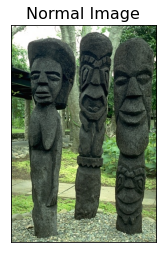
\includegraphics[width=\textwidth]{normal_compared.png}
        \caption{}
        \label{fig:f1}
      \end{subfigure}
      \hfill
      \begin{subfigure}[b]{0.19\textwidth}
        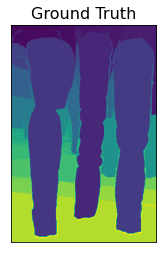
\includegraphics[width=\textwidth]{truth_compared.png}
        \caption{}
        \label{fig:f2}
      \end{subfigure}
      \hfill
      \begin{subfigure}[b]{0.19\textwidth}
        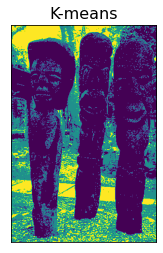
\includegraphics[width=\textwidth]{kmeans_compared.png}
        \caption{}
        \label{fig:f3}
      \end{subfigure}
      \hfill
      \begin{subfigure}[b]{0.19\textwidth}
        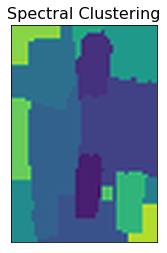
\includegraphics[width=\textwidth]{spectral_compared.png}
        \caption{}
        \label{fig:f4}
      \end{subfigure}
      \hfill
      \begin{subfigure}[b]{0.19\textwidth}
        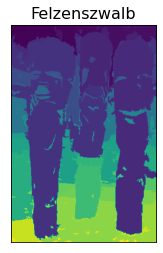
\includegraphics[width=\textwidth]{felzenszwalb_compared.png}
        \caption{}
        \label{fig:f5}
      \end{subfigure}
      \caption{Comparison of Segmentations}
    \end{figure}

    In the Figure 1, a sample image was chosen and the segmentations computed
    for each algorithm. At first glance, K-means seems to have performed well,
    but upon closer inspection the segments are not separated. The segments are 
    defined by their color with a different color indicating a different
    segmentation. K-means however, creates clusters solely based on color and 
    not by location, so similar colors are grouped together even if they are
    far apart or not even connected. This shows the importance that distance
    plays on producing accurate segmentations. A popular advancement to this
    is called SLIC which uses K-means on a 5D color space and pixel coordinates.
    \\
    \\
    Spectral clustering, performed well in creating segments based on distance,
    but fails when longer segments are needed. Certain edges can be seen in the
    segmentation, but they are broken up by other segments, leaving inaccurate
    results. Felzenszwalb performed the best of the three, but smaller
    segments within larger ones as well as oversegmentation leads to 
    inaccuracies.


  \section{Training Results}

    \begin{figure}[!h] %!tbp
      \begin{subfigure}[b]{0.5\textwidth}
        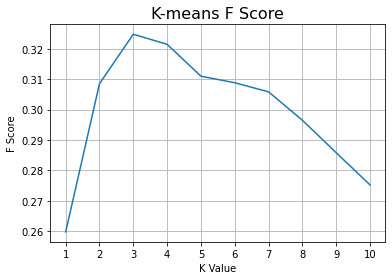
\includegraphics[width=\textwidth]{kmeans_score.png}
        \caption{}
        \label{fig:f1}
      \end{subfigure}
      \hfill
      \begin{subfigure}[b]{0.5\textwidth}
        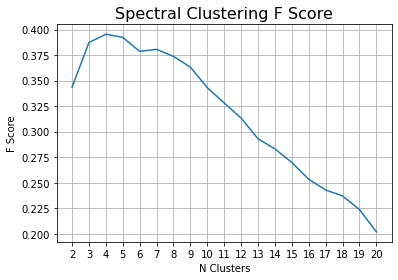
\includegraphics[width=\textwidth]{spectral_score.png}
        \caption{}
        \label{fig:f2}
      \end{subfigure}
      \hfill
      \begin{subfigure}[b]{\textwidth}
        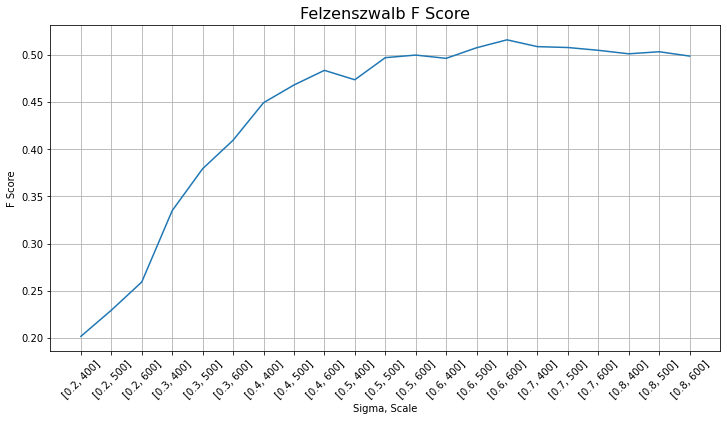
\includegraphics[width=\textwidth]{felzenszwalb_score.png}
        \caption{}
        \label{fig:f3}
      \end{subfigure}
      \caption{Training F-scores}
    \end{figure}

    Figure 2 shows the results of training the algorithms on a range of
    parameters and comparing them to the F-score. For both K-means and 
    spectral clustering it appears that a lower $k$ value provides better
    segmentations, with larger values leading to oversegmentation.
    Felzenszwalb was ran with 2 parameters, $\sigma$ and $scale$, defined in 
    section 2.3. As can be seen from the graph, higher values provides a 
    significantly higher F-score. This is likely due to the fact that a higher
    scale creates larger segments, which is necessary to match human drawn
    segmentations.

    \newpage

  \subsection{Test Accuracy and Time}

    \begin{table}[h!]
      \begin{tabular}{lllll}
      \hline
      Algorithm           & F-score & Testing Time (seconds) & Training Time (seconds) &  \\ \hline
      K-Means             & 0.3156  & 31.98                  & 1412.43                 &  \\
      Spectral Clustering & 0.3837  & 22.12                  & 1155.29                 &  \\
      Felzenszwalb        & 0.4633  & 9.47                   & 475.29                  &  \\ \hline
      \end{tabular}
      \caption{F-scores and Runtimes by Algorithm}
    \end{table}

    In Table 1, the results during training were reflected well in testing, except for Felzenszwalb
    which was about 0.05 less compared to training. Still, Felzenszwalb
    performed much better than the other two, with K-means performing the worst.
    This shows how significant the location of pixel values are when performing
    image segmentation. When compared to the results from other algorithms
    \cite{performance}, K-means and spectral clustering performed worse than
    the baseline random segmentation. However, it is important to note that 
    the actual benchmark was not performed, so discrepancies are likely when
    compared to these algorithms. Felzenszwalb performed fairly well, coming
    close to the 12th algorithm in the list. As for the runtime of the algorithms,
    Felzenszwalb again performed much better even with a larger range of
    parameters tested. K-means performed the slowest even with half the range 
    of parameters as the other two.


\section{Conclusions}

  Overall, Felzenszwalb performed better on all fronts compared to the K-means
  and Spectral Clustering. It also proved to be a competitive algorithm on
  the Berkeley Segmentation Dataset \cite{dataset}. This project was also 
  a great demonstration on the importance of pixel location for producing
  accurate segments and the effect of a graph based approach to segmentation. 
  These results and methods can be further used to train/test other algorithms
  in preparation for submission to Berkeley's Benchmarking software, since 
  the benchmark takes around 2 hours to complete. This paper also provides 
  decent hyperparameters for each of the algorithms listed, allowing further
  experimentation to improve them.

  \hfill

\bibliographystyle{unsrt}
\bibliography{references}

\end{document}
